\documentclass[a4paper]{report}

\usepackage{graphicx}
\graphicspath{{./images/} }

\title{Vaja 34 Hitrost zvoka v plinu}
\author {Jure Kos}
\date {4.1.2022}

\begin{document}
\maketitle

\chapter*{Uvod}

S pomočjo določanja lastnih frekvenc stoječega valovanja sem poskušal določiti hitrost zvoka. Lastno frekvenco se je določalo na dva načina - 1. način je bilo opazovanje poskakovanja žagovine v nastalih vozlih steklene cevi, 2. način pa je bilo storjeno s pomočjo odčitavanja voltmetra, na katerega je bil vezan mikrofon.

\section*{Naloga}
Določi hitrost zvoka v zraku z merjenji razmikov med vozli stoječega valovanja ter z opazovanjem frekvenčnih razmikov posameznih akustičnih resonanc v cevi. Izračunaj tudi adiabatno stisljivost plina.



\section*{Potrebščine}

\begin{itemize}
\item cev
\item zvočnik
\item frekvenčni generator
\item mikrofon
\item voltmeter
\end{itemize}







\chapter*{Navodila}

Vključimo generator frekvenc in spreminjamo frekvenco in poiščemo prvo stoječe valovanje plina v cevi.
Postopoma povečujemo frekvence in pri vsakem stoječem valovanju izmerimo razdaljo med dvema vozloma.
Iz razmikov med vozli določimo valovno dolžino in posledično hitrost zvoka. Ponovno se sprehodimo čez frekvence
in si zapišemo vrednosti pri katerih se pojavijo akustične resonance. Iz dobljenih frekvenc za njih izračunamo hitrost zvoka.
Po formuli za adiabatno stisljivost zraka, jo izračunamo:

\begin{equation}
  c = \sqrt{\frac{1}{\chi_s \rho}}
\end{equation}


\section*{Skica}

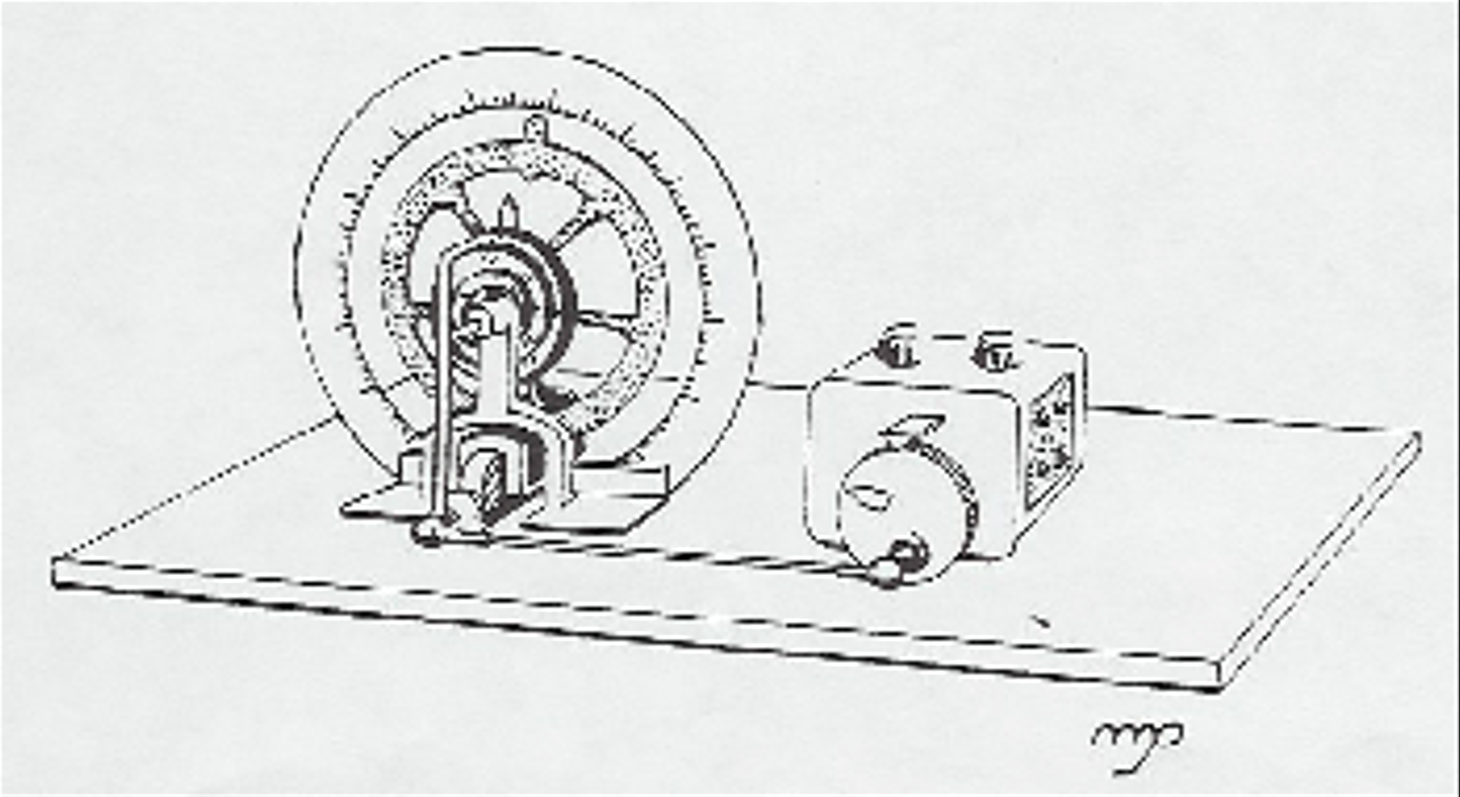
\includegraphics[width=\textwidth]{Skica}



\chapter*{Meritve in hitrost zvoka}

\begin{center}
  \begin{tabular}{| c | c | c |}
    \hline
    Stoječe valovanje & Frekvenca $\nu$ [Hz] & Valovna dolžina $\delta$ [$m$] \\ \hline
    1 & 118 & 0,78$\pm 5cm$ \\ \hline
    2 & 260 & 0,61$\pm 3cm$ \\ \hline
    3 & 430 & 0,39$\pm 3cm$ \\ \hline
    4 & 550 & 0,28$\pm 3cm$ \\ \hline
    5 & 680 & 0,25$\pm 2cm$ \\ \hline
    6 & 795 & 0,22$\pm 1cm$ \\ \hline
    7 & 960 & 0,18$\pm 1cm$ \\ \hline
    8 & 1120 & / \\ \hline
    9 & 1295 & / \\ \hline
    10 & 1460 & / \\ \hline
    11 & 1605 & / \\ \hline

  \end{tabular}
\end{center}

\noindent Dolžina cevi = $0.97m \pm 3mm$

\section*{Hitrost zraka z merjenjem razmikov med vozli}

Graf rezultatov:

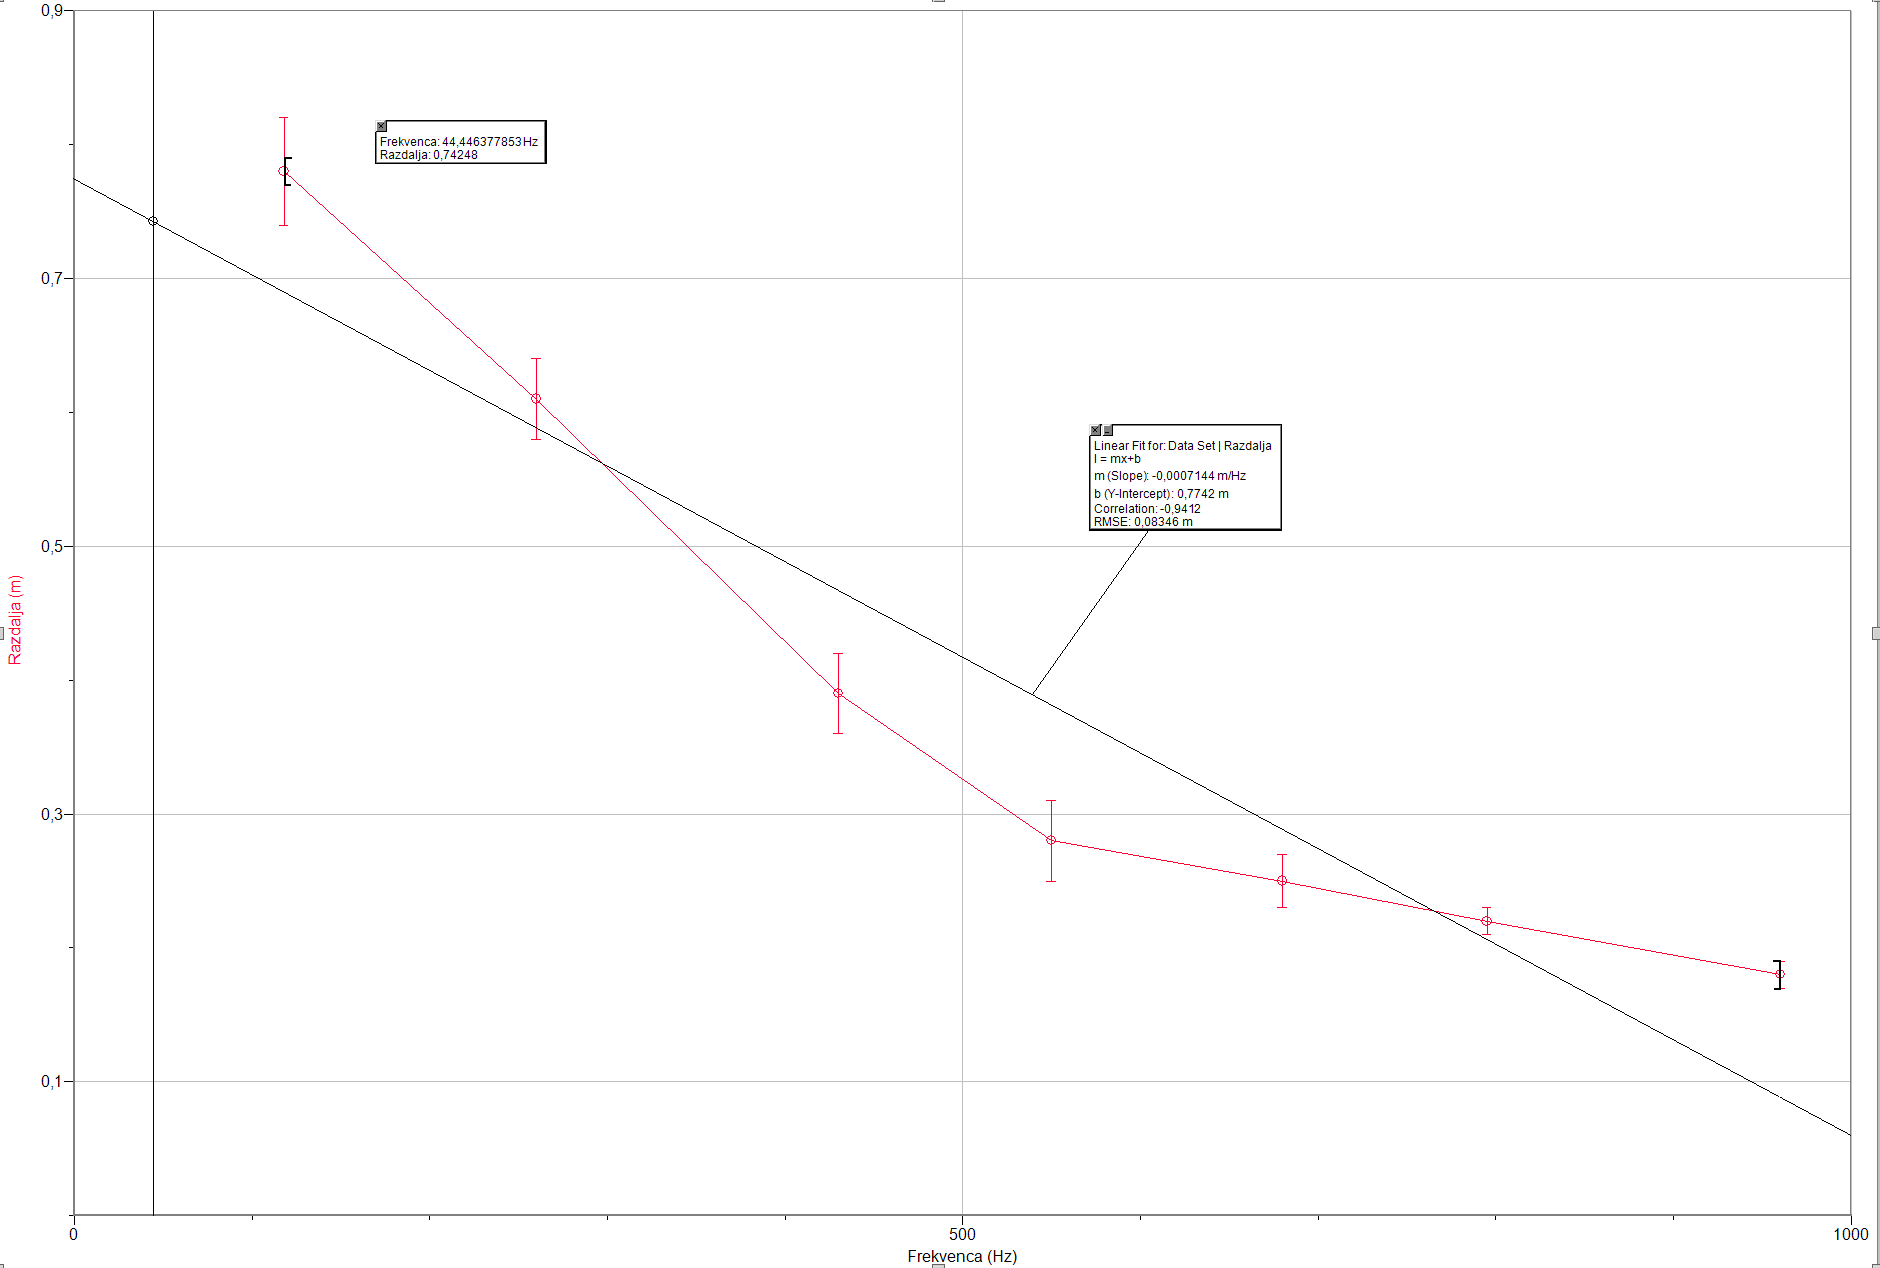
\includegraphics[width=\textwidth]{Lambda}

\noindent Iz ploščine grafa med premico in koordinatnima osema lahko določimo hitrost zvoka:\\
Vrednost $y$ pri sekanju ordinatne osi: $y = 0,77m \pm 0,05m$ \\
Vrednost $x$ pri sekanju abcisne osi: $x=1022Hz \pm 5Hz$

\noindent Hitrost zvoka:

\begin{equation}
  c = \frac{yx}{2} = \frac{1022Hz(1 \pm 0,005 ) \cdot 0,77(1 \pm 0,06)m}{2} = 390m/s\pm 30m/s  
\end{equation}

\section*{Hitrost zvoka z akustičnimi frekvencami}

Graf rezultatov:

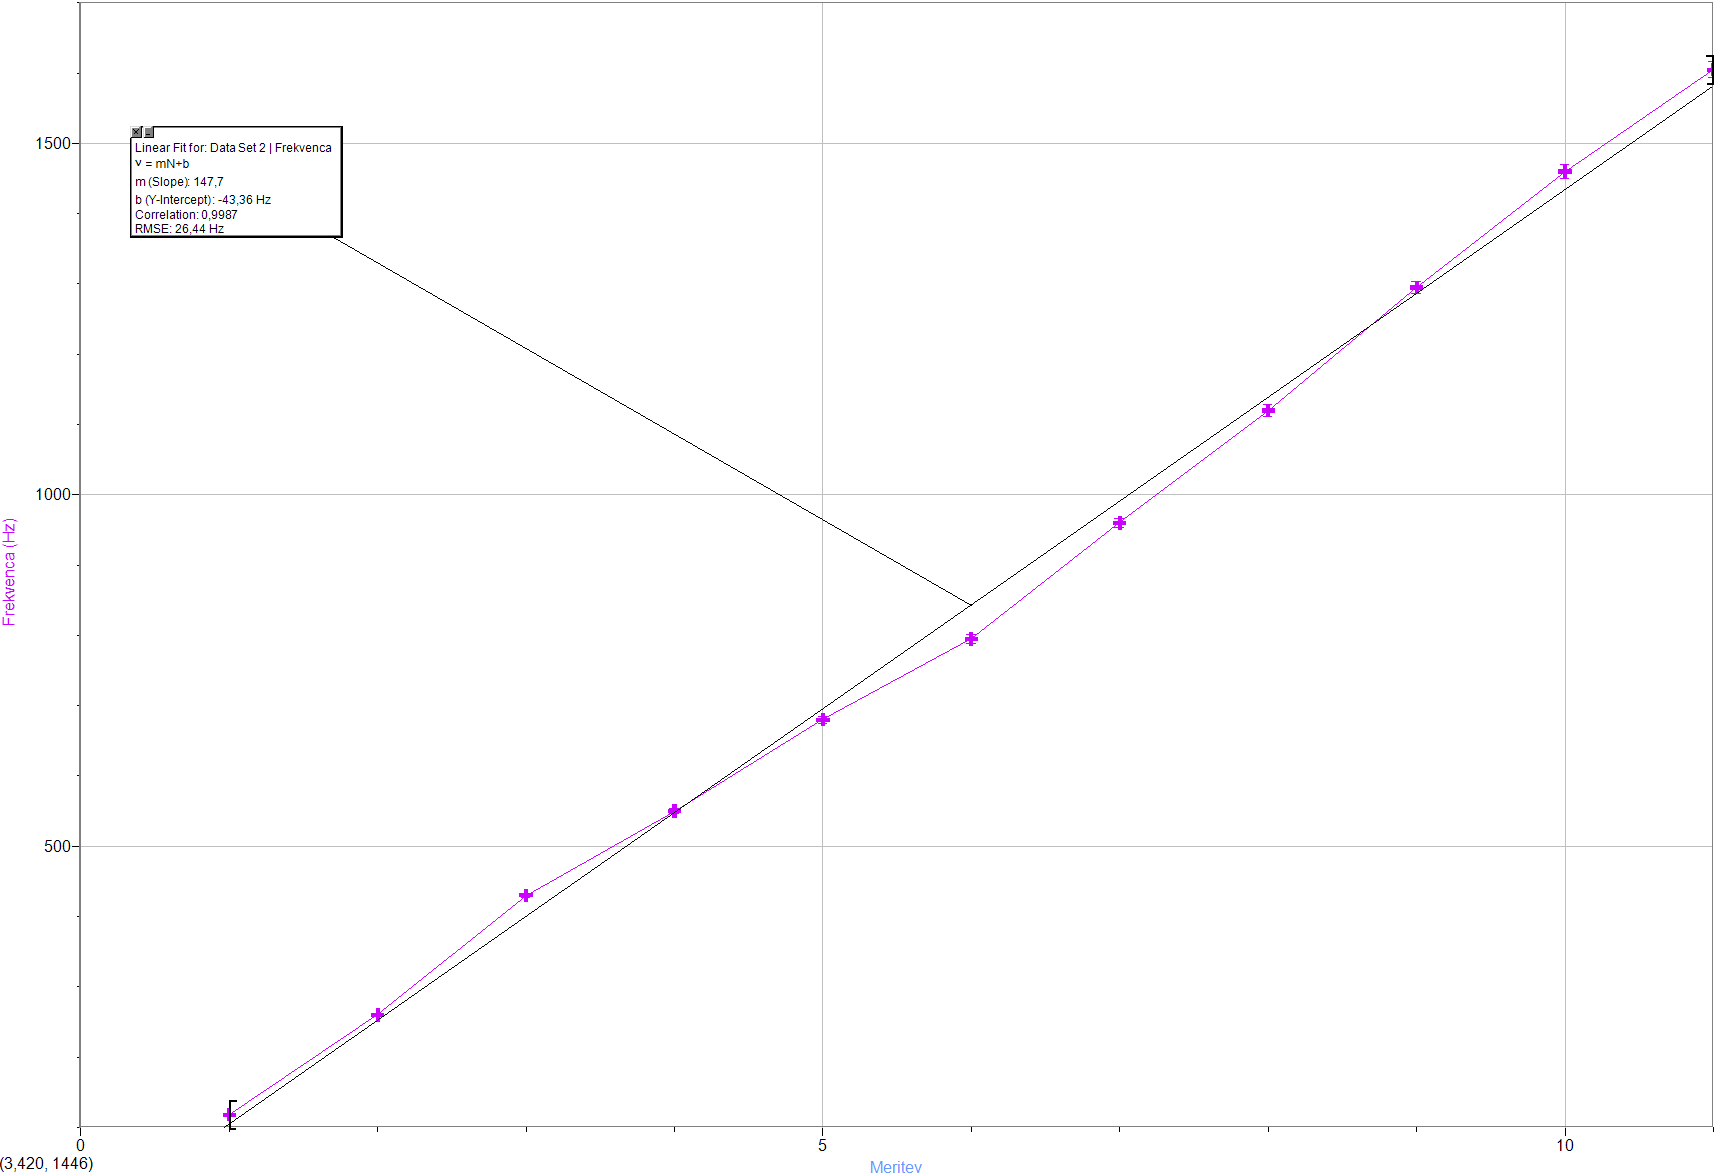
\includegraphics[width=\textwidth]{Frekvence}

\noindent Iz naklona premice in enačbe določimo hitrost zvoka. \\
Naklon premice: \\

  \[k =147,7 (1 \pm 0,01) s^{-1}\]

\noindent Hitrost zvoka:
\begin{equation}
  c = 2lk = 2 \cdot 0,97(1 \pm 0,003)m \cdot 147,7(1 \pm 0,01)s^{-1} = 275m/s \pm 10 m/s
\end{equation}
  


\chapter*{Adiabatna stisljivost zraka}

\section*{Razmiki:}

\begin{equation}
  \chi_s = \frac{1}{c^2 \rho} = \frac{1}{(390 m/s)^2 \cdot 1.2 kg/m^3} = 5,5 \cdot 10^{-6} (1 \pm 0,14) m/kgs^2
\end{equation}

\section*{Akustične frekvence:}

\begin{equation}
  \chi_s = \frac{1}{c^2 \rho} = \frac{1}{(275 m/s)^2 \cdot 1.2 kg/m^3} = 1,1 \cdot 10^{-5} (1 \pm 0,05)m/kgs^2
\end{equation}


\end{document}